\documentclass[10pt]{article}
\usepackage[margin=0.72in]{geometry}
\usepackage{graphicx,booktabs,amsmath,amssymb,hyperref,caption,subcaption,float,xcolor,longtable}
\hypersetup{colorlinks=true,linkcolor=blue,urlcolor=blue,citecolor=blue}
\title{Technical Report: 30B-Token FinalArchitecture Transformer++ Training Run}
\author{Artifact-derived analysis of the selected Blob run}
\date{Generated from the completed run artifacts}
\begin{document}
\maketitle

\begin{abstract}
This report analyzes the completed 30B-token training run identified in the artifact inventory. The run trained a 150.44M-parameter ternary Transformer++ for 30.000B cumulative tokens and exited with code 0. The final held-out loss was 2.1653 nats (perplexity 8.717); the best scheduled validation loss was 2.0641 at step 252000. Attention telemetry remained finite: its largest sampled absolute logit was 7.761, while the final sampled maximum was 7.548. The run was numerically stable under the logged observables, but its final relative ternary reconstruction MSE was 0.426. The configuration contains no numerical pass/fail threshold for this quantity, so the artifacts establish the measurement but do not establish a formal MSE gate pass.
\end{abstract}

\section{Run identity and evidence boundary}
This paper uses only the Blob-synced artifacts in the source mirror named by the run identifier recorded in \texttt{RUN\_ID.json}. Identity is supported by the resolved cumulative token count (29,999,996,928), the final checkpoint at step 261,580, the final milestone record, and \texttt{exit\_code.txt}. The run resumed from step 33,136; the reporting series therefore includes the full cumulative trajectory through the final step rather than treating the resumed segment as an independent experiment. All figures were generated by \texttt{generate\_report.py} from the mirrored JSON/JSONL files. Machine-readable tables are emitted in \texttt{tables/}.

\section{Setup discovered from run artifacts}
The model configuration reports 20 Transformer layers, hidden width 768, 12 query heads, 4 KV heads, and FFN width 2048. A parameter-count audit of this exact configuration gives 150,436,648 trainable parameters: 125,829,120 BitLinear matrix parameters and 24,607,528 embedding/norm parameters. The attention policy is sixteen local layers and four global layers: global layers $\{4,9,14,19\}$ and a local window of 1024 tokens. The sequence length is 4096; the global-to-local layer ratio is 1:4.

\begin{table}[H]\centering
\caption{Discovered training configuration.}\label{tab:setup}
\begin{tabular}{ll}\toprule
Item & Recorded value \\\midrule
Tokenizer & \texttt{TinyLlama/TinyLlama-1.1B-Chat-v1.0}, revision \texttt{fe8a4ea1ffed...66a451e6} \\
Precision / device & BF16 on NVIDIA H100 NVL (99.5 GB) \\
Batch / sequence / tokens per step & 28 / 4096 / 114,688 \\
Total budget / final step & 30.000B tokens / 261,580 \\
Attention & FA3; local window 1024; globals 4, 9, 14, 19 \\
Normalization & unit-RMS Q/K before RoPE; SubLN enabled; residual init scale 1.0 \\
Weight quantization & deterministic grouped absmean; group size 128; activation quantization disabled \\
Optimizers & Muon for BitLinear matrices; AdamW for embeddings and RMSNorm weights \\
Base learning rates & Muon 0.0030; AdamW 0.0030; norm 0.0002 \\
Schedule / decay & cosine; warmup 10.0\%; terminal LR fraction 0.10 \\
Weight decay & Muon 0.10; AdamW 0.10 \\
\bottomrule\end{tabular}
\end{table}

The data manifest defines the following phase-wise mixture: phase\_1: 5B tokens; nemotron\_cc\_hqsynth 40.0\%, pretraining\_corpus 20.0\%, cosmopedia\_v2\_mincols 40.0\%\\ phase\_2: 15B tokens; nemotron\_cc\_hqsynth 70.0\%, cosmopedia\_v2\_mincols 30.0\%\\ phase\_3: 10B tokens; nemotron\_cc\_hqsynth 12.5\%, fineweb\_edu 30.0\%, cosmopedia\_v2\_mincols 17.5\%, pretraining\_corpus 40.0\%. Phase boundaries at 5B and 20B cumulative tokens are marked in Figs.~\ref{fig:global}--\ref{fig:quant}.

\section{Global training dynamics}
Figure~\ref{fig:global} separates raw batch loss from the logged running loss and held-out validation loss. The first logged batch loss was 10.8749; the final logged batch loss was 1.8892; the final running loss was 1.8370. Held-out validation fell from 3.8924 at step 2,000 to 2.1463 at the final scheduled validation step 260,000. The best scheduled value was 2.0641 at step 252,000; the final milestone value was 2.1653, 4.90\% above that best point. This late increase is measured, but the logs do not contain a causal annotation that permits attribution to a specific data component or schedule event.

The global gradient norm declined from 7.511 at the first logged step to 0.208 at the final logged step. Its maximum, 8.260, occurred at step 5. The highest raw batch loss, 10.903, occurred at step 5; the minimum, 1.462, occurred at step 221,000. There is no logged NaN/Inf event in the analyzed series. The realized matrix learning rates in Fig.~\ref{fig:global} are larger than the base Muon LR because the recorded RMS-matching multiplier is applied per matrix.

\begin{figure}[H]\centering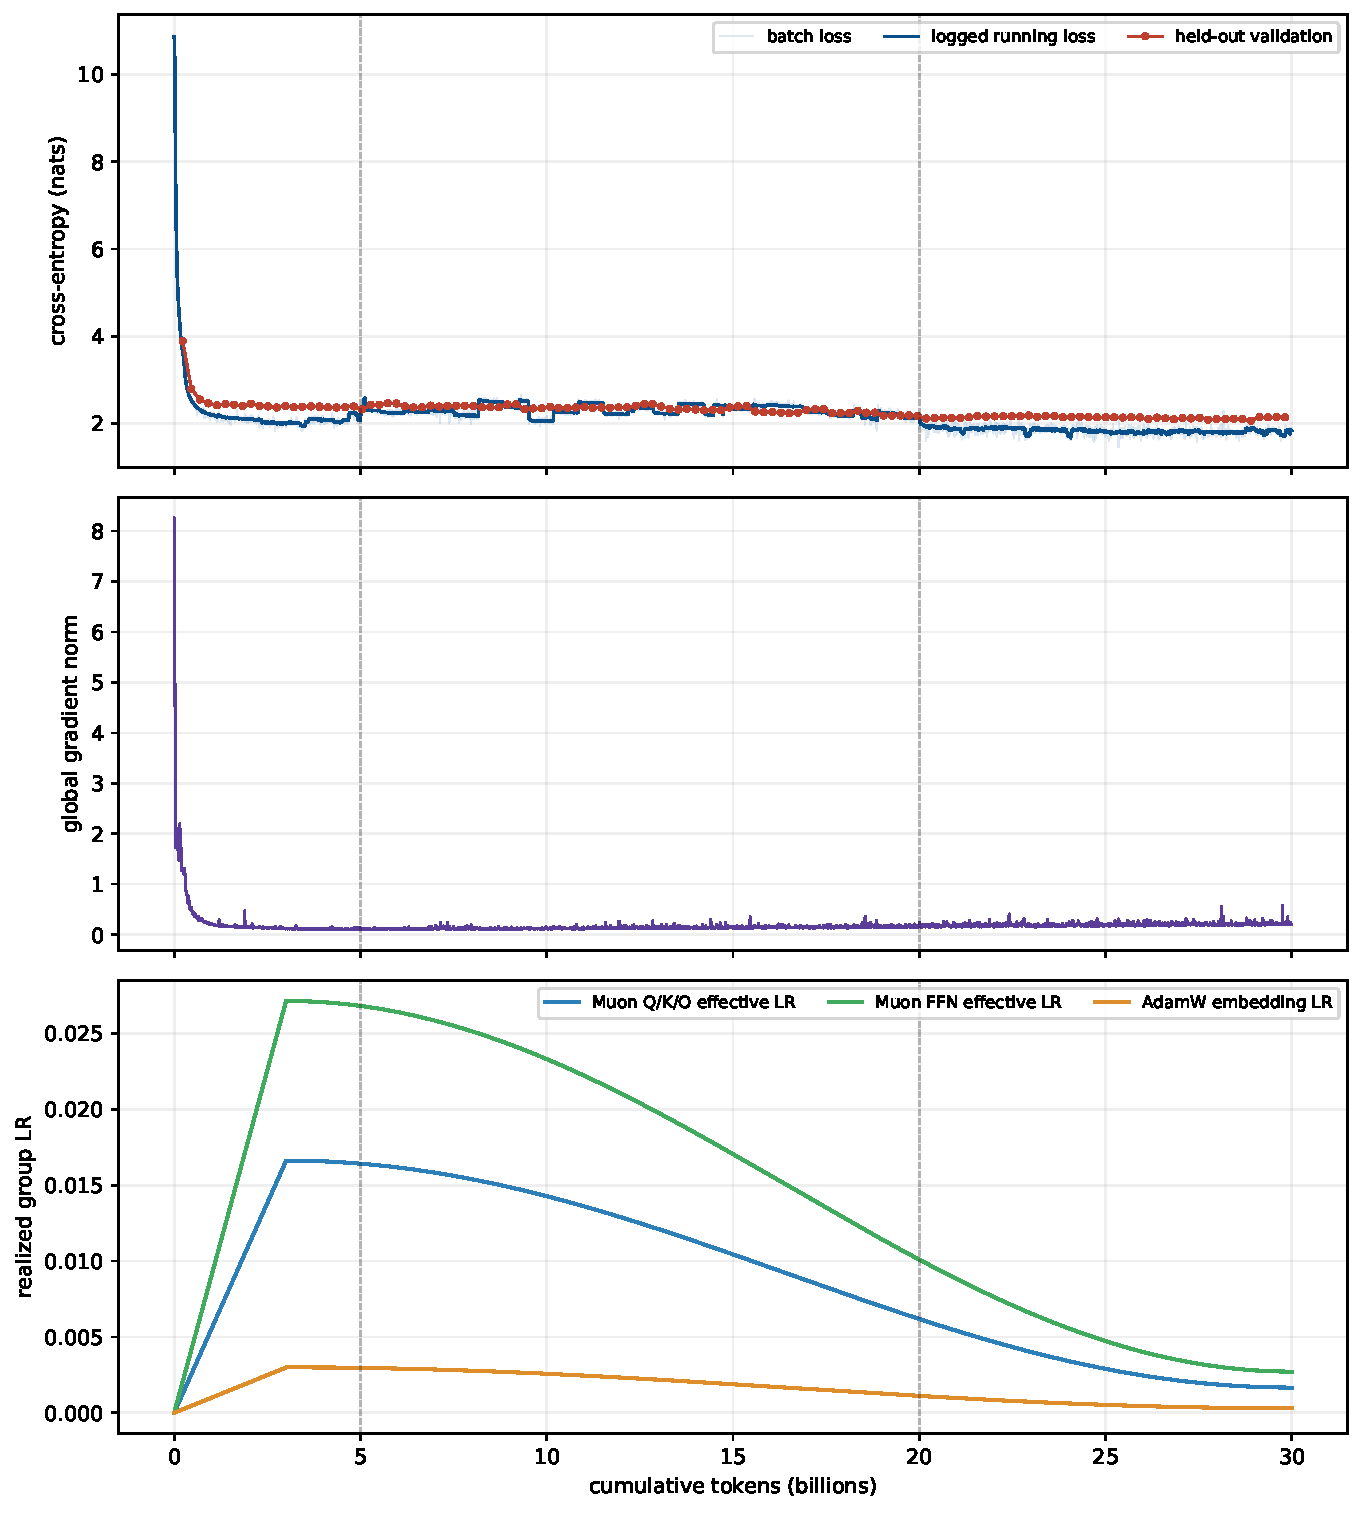
\includegraphics[width=\linewidth]{figures/global_training_dynamics.pdf}
\caption{Loss, gradient norm, and realized optimizer-group learning rates across the full cumulative trajectory. Dashed vertical lines mark the 5B- and 20B-token curriculum boundaries.}\label{fig:global}
\end{figure}

\section{Quantization and numerical stability}
The model uses ternary weight quantization and no activation quantization. Figure~\ref{fig:quant} reports the logged reconstruction series. Relative MSE increased from 0.261 at the first quantified point to 0.426 at the final exhaustive milestone measurement; final absolute MAE was 0.0443. The final ternary distribution was $p(-1)=0.308$, $p(0)=0.383$, and $p(+1)=0.309$, with normalized ternary entropy 0.99498. The final flip-rate EMA was 0.261.

The configuration sets \texttt{max\_quantization\_relative\_mse=null}, \texttt{min\_ternary\_zero\_fraction=null}, and \texttt{max\_ternary\_zero\_fraction=null}. Consequently, the artifact record contains no numerical quantization gate. The measured final relative MSE of 0.426 is therefore \emph{not formally classifiable as pass or fail} from this run alone.

The decomposition records an oracle relative MSE of 0.248, scale-gap contribution 0.058, support-gap contribution 0.117, and identifies \texttt{irreducible} as the largest component. The module-health scan attributes 89.1\% of mean reconstruction error to weights with magnitude above $1.5\alpha$, while zero-cell error contributes 5.3\%. These are reconstruction diagnostics, not evidence of non-finite numerical behavior.

\begin{figure}[H]\centering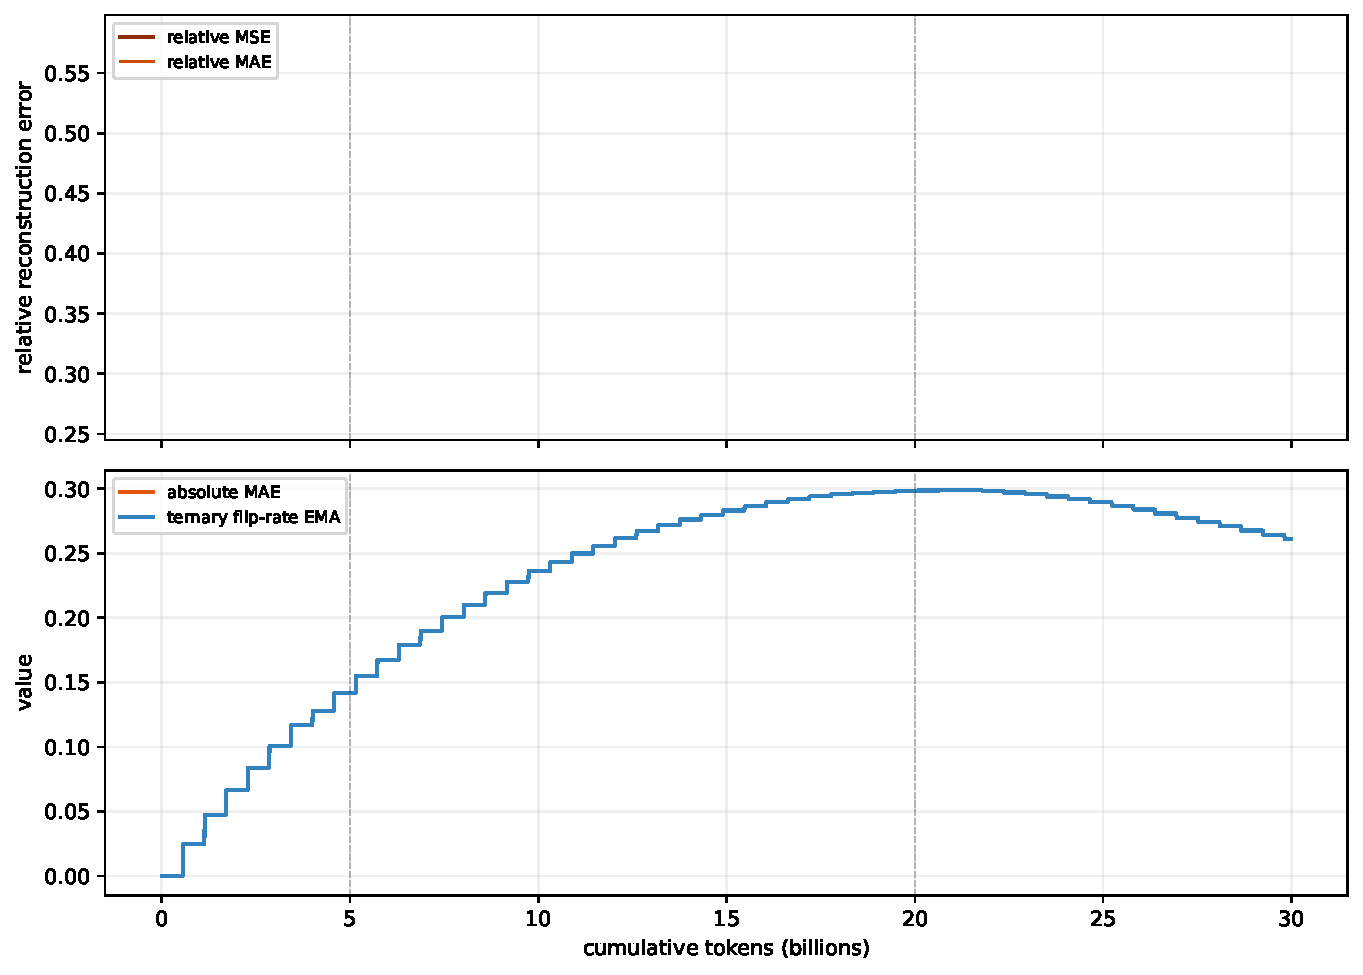
\includegraphics[width=\linewidth]{figures/quantization_dynamics.pdf}
\caption{Logged quantization error and ternary flip dynamics. No MSE or occupancy threshold was configured, so no line is drawn as a pass/fail gate.}\label{fig:quant}
\end{figure}

\section{Layerwise analysis}
All 20 layers are represented in the telemetry, not only the top-layer summary. Figure~\ref{fig:attheat} shows the complete 52-snapshot layer-by-time logit and entropy matrices. The largest sampled absolute logit across the run was 7.761; it occurred before the final snapshot. The final snapshot at step 260,000 has maximum sampled absolute logit 7.548, mean normalized entropy 0.646, and minimum layer entropy 0.580. Every logged layer reports finite-logit fraction 1.0 and zero non-finite logits.

At the final snapshot, layer 10 (local) has the largest sampled absolute logit, 7.548. Layer 16 (local) has the lowest normalized entropy, 0.580. Layer 15 has the largest near-one-hot query fraction, 2.54\%. These are not a sink diagnosis: the telemetry contains no explicit sink-token metric, and the sampled low-entropy fraction stays below 1\% in every final layer. Post-RoPE Q and K vector RMS values remain close to 1.0 by construction and are displayed in Fig.~\ref{fig:attfinal}.

\begin{figure}[H]\centering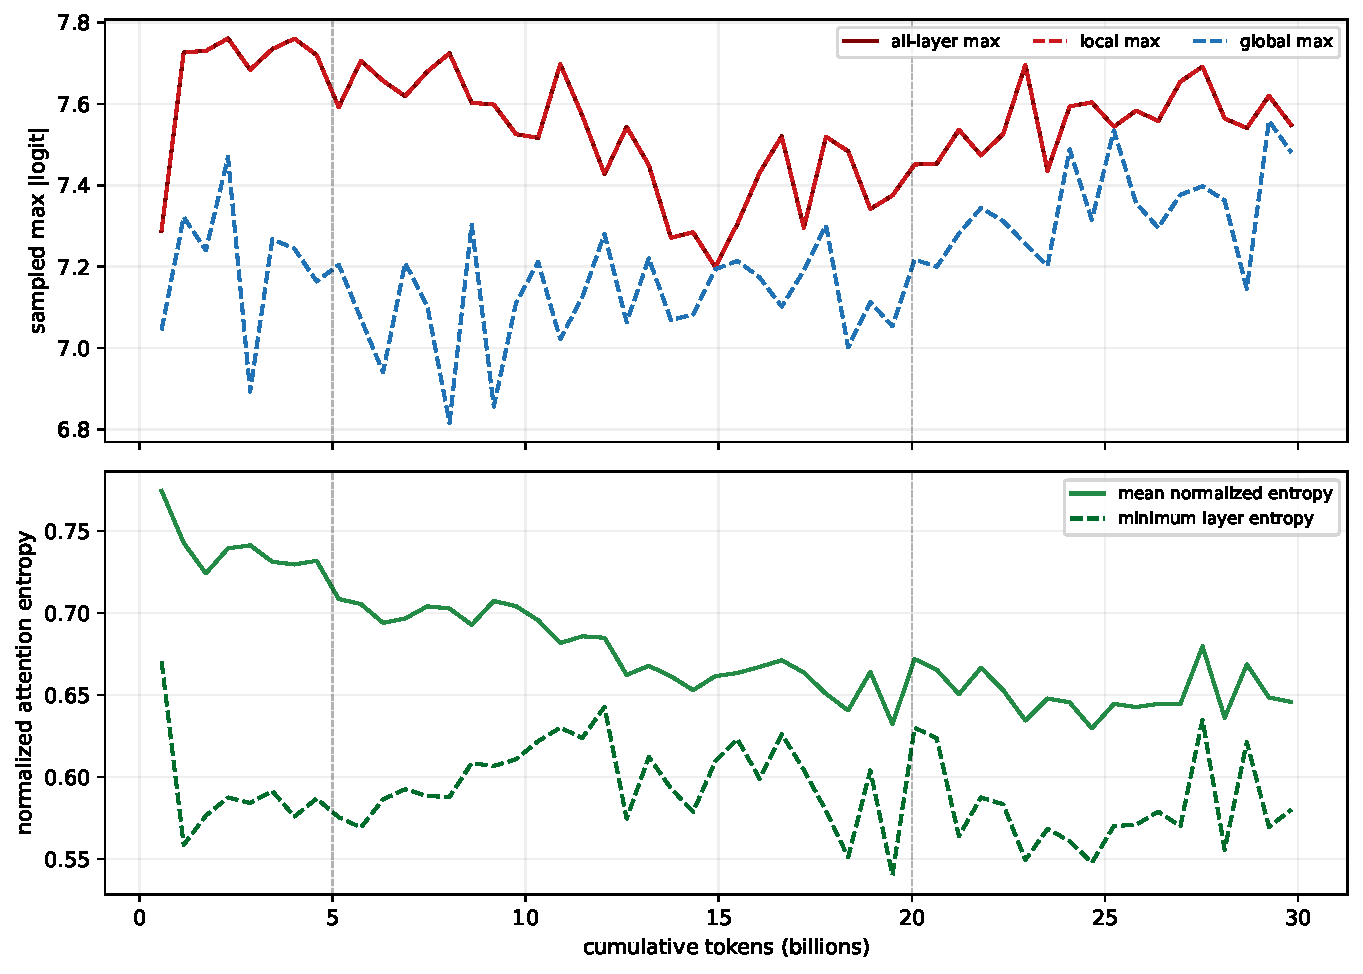
\includegraphics[width=\linewidth]{figures/attention_global_dynamics.pdf}
\caption{Aggregate attention telemetry over time.}\label{fig:attglobal}
\end{figure}
\begin{figure}[H]\centering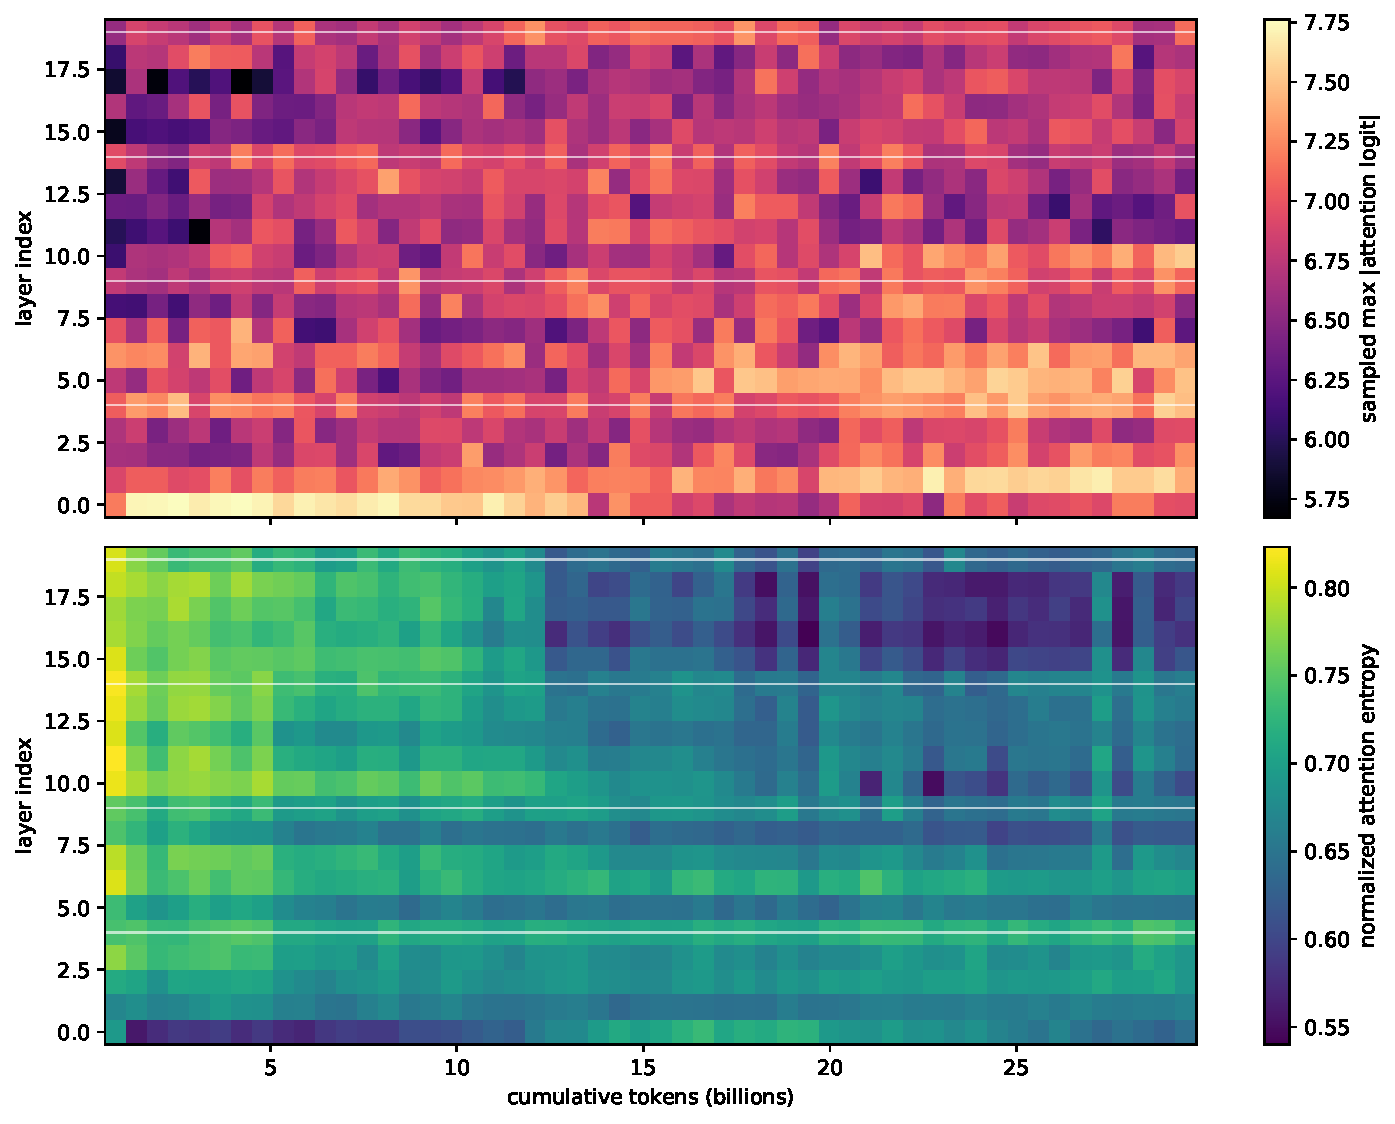
\includegraphics[width=\linewidth]{figures/attention_layerwise_heatmaps.pdf}
\caption{Full layer-by-time attention telemetry. White horizontal guides identify global layers.}\label{fig:attheat}
\end{figure}
\begin{figure}[H]\centering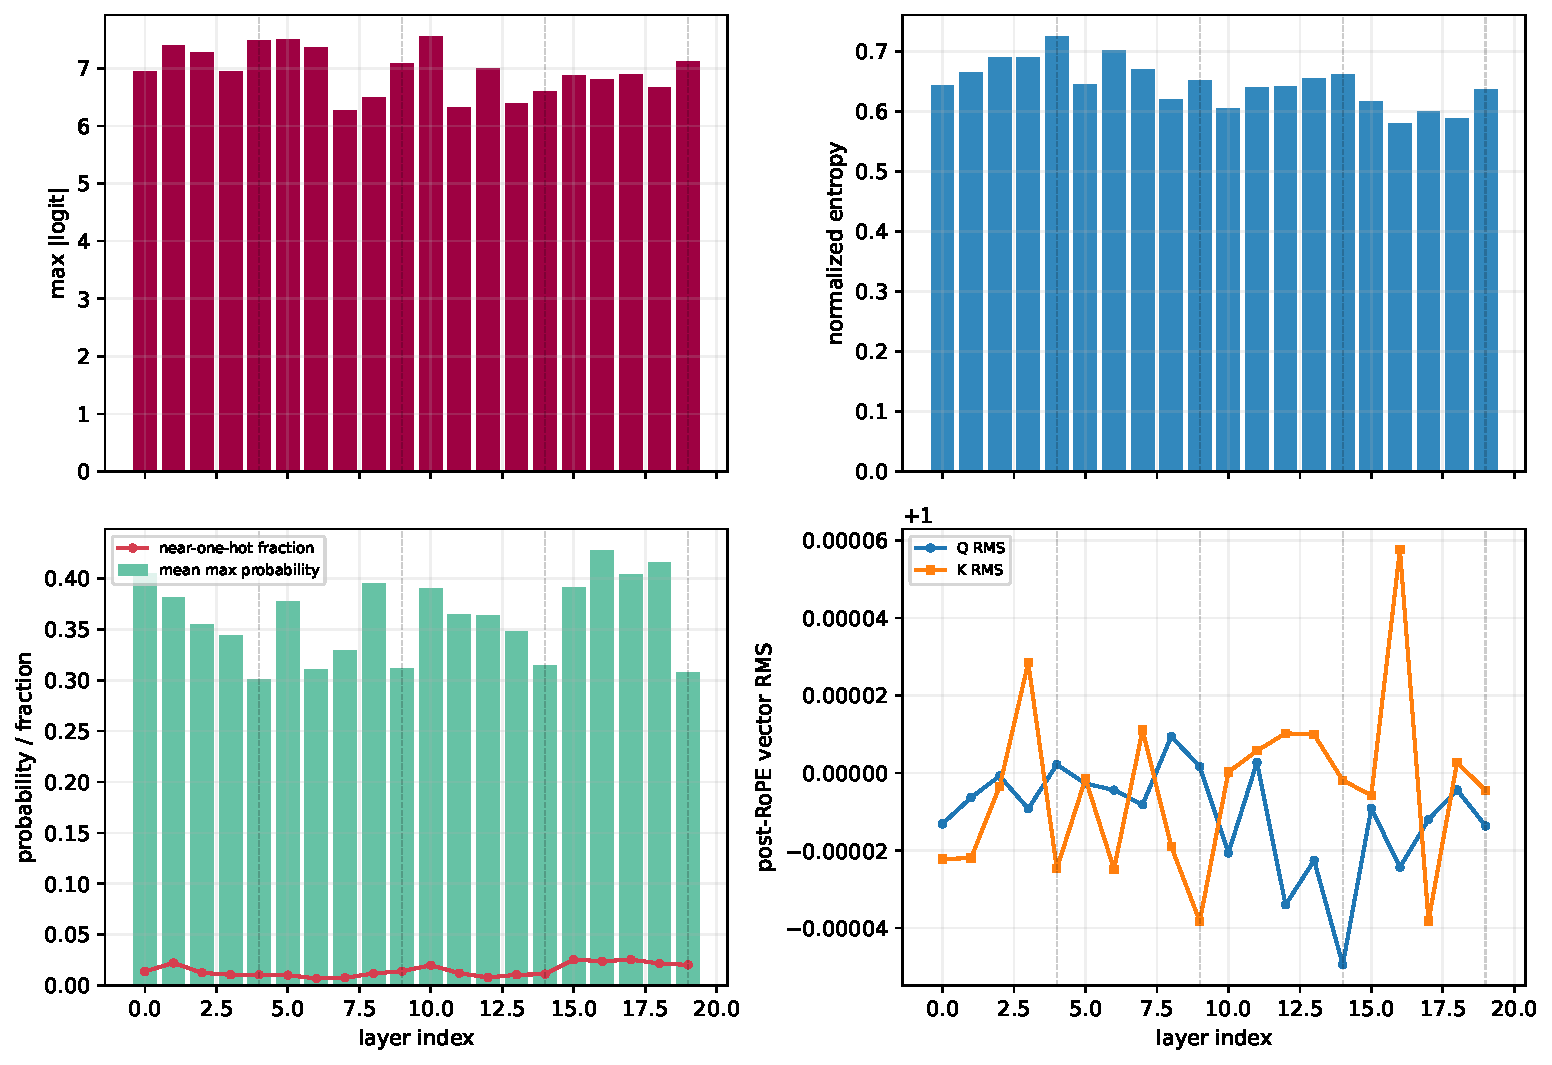
\includegraphics[width=\linewidth]{figures/final_layerwise_attention.pdf}
\caption{Final sampled layerwise attention statistics at step 260,000.}\label{fig:attfinal}
\end{figure}

Figure~\ref{fig:updates} aggregates every BitLinear matrix within each layer with parameter-count weighting. At the last update-stat snapshot (step 260,000), layer 1 has the largest update-to-weight RMS ratio (0.000808). This is an update-scale outlier, not a divergence signal: the full layerwise maximum remains below $10^{-3}$ and all logged updates are finite. Weight RMS, update ratios, and sampled sign-change rates are shown for all layers in Fig.~\ref{fig:updates}.

\begin{figure}[H]\centering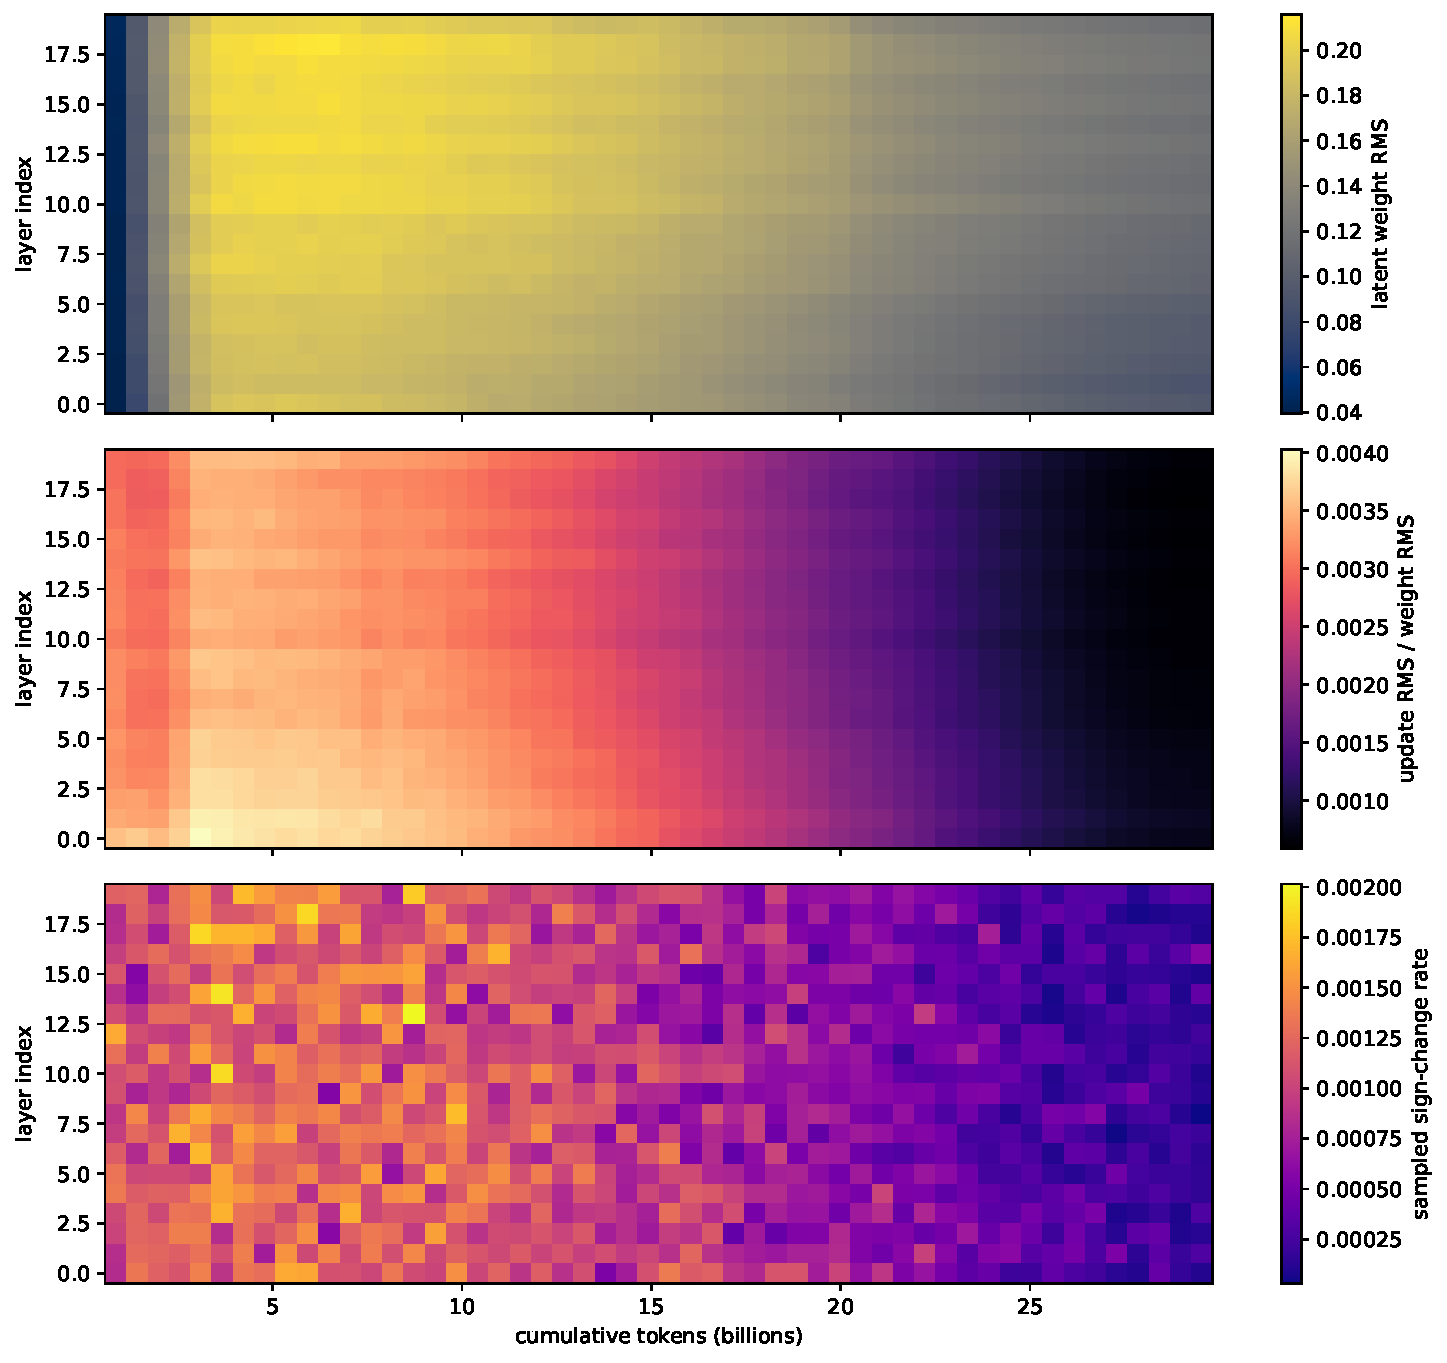
\includegraphics[width=\linewidth]{figures/layerwise_update_dynamics.pdf}
\caption{Parameter-count-weighted BitLinear update diagnostics by layer.}\label{fig:updates}
\end{figure}

The final quantization scan covers 125,829,120 weights. Layer 19 (global) has the largest aggregate relative MSE (0.446); layer 12 has the largest aggregate zero fraction (38.93\%). These are reconstruction outliers. They do not coincide with the largest attention logit, and the artifact does not log a causal linkage between reconstruction error and attention behavior.

\begin{figure}[H]\centering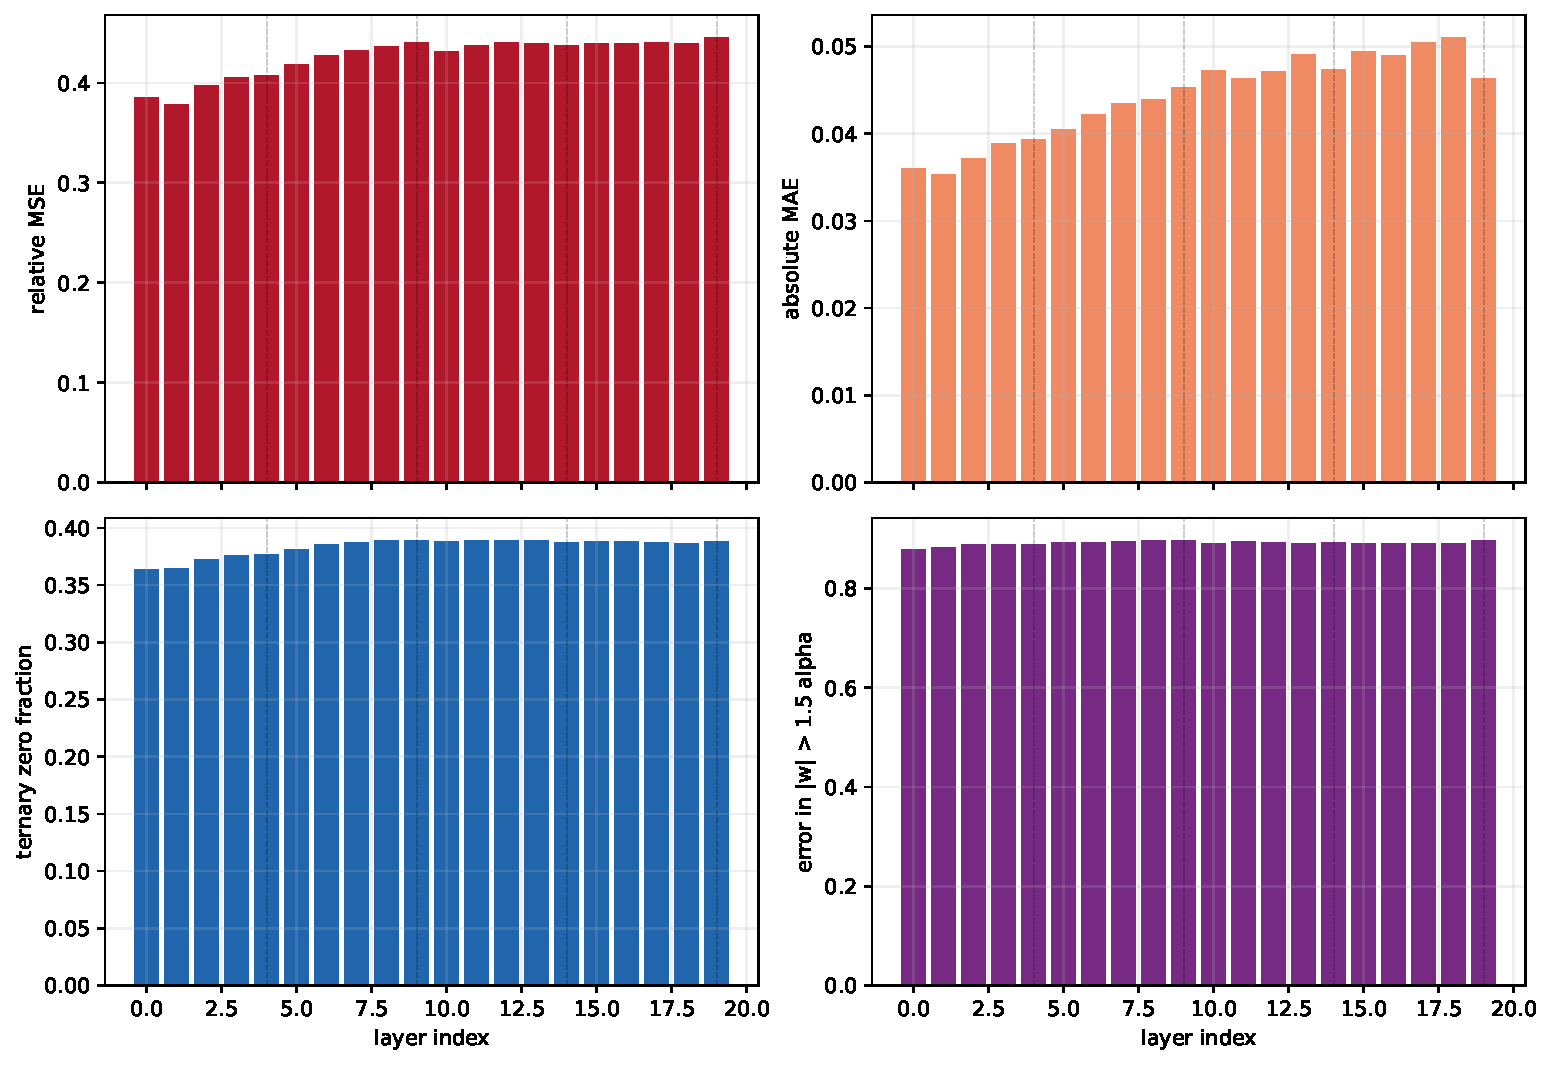
\includegraphics[width=\linewidth]{figures/final_layerwise_quantization.pdf}
\caption{Final full-scan, parameter-count-weighted quantization diagnostics by layer.}\label{fig:qfinal}
\end{figure}

\begin{table}[H]\centering
\caption{Final attention outliers from the full layerwise snapshot.}\label{tab:attout}
\begin{tabular}{lrrrrr}\toprule
Criterion & Layer & Kind & max $|z|$ & Entropy & near-one-hot \\\midrule
highest sampled logit & 10 & local & 7.548 & 0.604 & 1.99\% \\
lowest entropy & 16 & local & 6.810 & 0.580 & 2.38\% \\
highest near-one-hot fraction & 15 & local & 6.878 & 0.616 & 2.54\% \\
\bottomrule\end{tabular}
\end{table}

\section{Evaluation results}
Table~\ref{tab:eval} compares the final checkpoint with the preceding independently evaluated checkpoint at step 209,264. Both checkpoints were evaluated with the same checked-in model source hash and SDPA reference backend on an NVIDIA L40S. HellaSwag token-normalized accuracy, LAMBADA exact accuracy, ARC-Easy raw accuracy, and WinoGrande raw accuracy increased. SciQ raw accuracy decreased by 0.70 percentage points. The evidence supports mixed late-stage downstream movement, not a claim that every benchmark improved.

\begin{table}[H]\centering
\caption{Final checkpoint versus step-209,264 evaluation. Values are percentage points.}\label{tab:eval}
\begin{tabular}{llrrr}\toprule
Task & Metric & Step 209,264 & Final & $\Delta$ \\\midrule
hellaswag & token-normalized accuracy & 30.86 & 31.27 & +0.41 \\
lambada & exact accuracy & 22.36 & 23.68 & +1.32 \\
arc\_easy & raw accuracy & 27.65 & 27.74 & +0.08 \\
winogrande & raw accuracy & 51.93 & 52.41 & +0.47 \\
sciq & raw accuracy & 77.50 & 76.80 & -0.70 \\
\bottomrule\end{tabular}
\end{table}

\section{Discussion}
The logged numerical trajectory is stable in the limited, observable sense: the run completed with exit code 0; all sampled attention logits were finite; the maximum sampled absolute logit stayed in the interval [7.199, 7.761]; post-RoPE Q/K RMS stayed approximately one; and update-to-weight RMS remained below $10^{-3}$ at the final update snapshot. The data do not support calling the final phase strictly improving on held-out loss, because the best scheduled validation was 2.0641 and the final milestone was 2.1653.

Quantization reconstruction error remains the clearest unresolved scale risk: final relative MSE was 0.426, with 89.1\% of mean error assigned to the saturated tail. However, this run configured no numerical quantization gate, so a formal quality verdict cannot be inferred from MSE alone. Before a larger scale-up, the next run should preserve the current full layerwise attention telemetry and add an explicit, pre-registered quantization criterion with an allowed MSE/MAE range and a downstream-evaluation decision rule.

\section{Limitations}
The attention statistics are sampled over one batch and 256 evenly spaced sequence positions, not an exhaustive $4096\times4096$ matrix. There is no explicit sink-token counter, no per-layer activation norm for the FFN/residual stream, and no configured numerical MSE, zero-fraction, or attention-logit pass/fail threshold. Therefore this report can establish observed finiteness and layerwise sampled behavior, but cannot certify an unlogged sink absence, full-sequence attention distribution, or formal gate clearance.

\appendix
\section{Full final layerwise quantization table}
\begin{longtable}{rrrrrr}
\caption{Final full-scan, parameter-count-weighted layer metrics. The complete time-series CSV supplements are in \texttt{tables/}.}\\
\toprule Layer & Kind & rel. MSE & abs. MAE & zero frac. & tail-error frac. \\\midrule
\endfirsthead
\toprule Layer & Kind & rel. MSE & abs. MAE & zero frac. & tail-error frac. \\\midrule
\endhead
0 & local & 0.385 & 0.0360 & 36.34\% & 87.91\% \\
1 & local & 0.378 & 0.0353 & 36.46\% & 88.35\% \\
2 & local & 0.397 & 0.0371 & 37.26\% & 88.80\% \\
3 & local & 0.405 & 0.0388 & 37.57\% & 88.95\% \\
4 & global & 0.407 & 0.0393 & 37.69\% & 88.89\% \\
5 & local & 0.418 & 0.0405 & 38.10\% & 89.27\% \\
6 & local & 0.428 & 0.0422 & 38.53\% & 89.32\% \\
7 & local & 0.432 & 0.0434 & 38.71\% & 89.47\% \\
8 & local & 0.437 & 0.0440 & 38.88\% & 89.64\% \\
9 & global & 0.440 & 0.0453 & 38.93\% & 89.58\% \\
10 & local & 0.431 & 0.0473 & 38.84\% & 89.03\% \\
11 & local & 0.437 & 0.0464 & 38.90\% & 89.41\% \\
12 & local & 0.440 & 0.0471 & 38.93\% & 89.34\% \\
13 & local & 0.439 & 0.0490 & 38.92\% & 89.15\% \\
14 & global & 0.437 & 0.0473 & 38.75\% & 89.28\% \\
15 & local & 0.440 & 0.0494 & 38.84\% & 89.05\% \\
16 & local & 0.439 & 0.0490 & 38.84\% & 89.14\% \\
17 & local & 0.441 & 0.0504 & 38.75\% & 89.04\% \\
18 & local & 0.439 & 0.0511 & 38.68\% & 88.97\% \\
19 & global & 0.446 & 0.0463 & 38.86\% & 89.73\% \\
\bottomrule
\end{longtable}

\section{Artifact inventory}
The report was generated from \texttt{configs/model\_config.json}, \texttt{configs/train\_config.json}, \texttt{configs/data\_manifest.json}, \texttt{configs/resolved\_budget.json}, \texttt{configs/environment.json}, \texttt{logs/train.jsonl}, \texttt{logs/validation.jsonl}, \texttt{logs/attention.jsonl}, \texttt{logs/dynamics.jsonl}, \texttt{milestones/final/metrics.json}, and the final and step-209,264 evaluation result files. The generated files \texttt{tables/training\_timeseries.csv}, \texttt{tables/final\_attention\_layers.csv}, \texttt{tables/final\_quantization\_layers.csv}, and \texttt{tables/layerwise\_update\_timeseries.csv} are the machine-readable raw tables underlying the figures.
\end{document}
